\documentclass[11pt, oneside, numbers=noenddot]{scrbook}
\usepackage{amstex}
\input{./includes/htl_definintions}

% Initialen der Authoren
\newcommand{\authorInitialsA}{TD} % Tobias Daxecker
\newcommand{\authorInitialsB}{MS} % Mathias Standhartinger

% Die Initialen werden verwendet um anzuzeigen wer welches Kapitel
% erstellt hat.

% Die Befehle \authorA - \authorB werden in den Kapitelüberschriften angefügt
\newcommand{\authorA}{\textmd{\textsuperscript{\authorInitialsA}}}
\newcommand{\authorB}{\textmd{\textsuperscript{\authorInitialsB}}}

% Titel der Arbeit:
\newcommand{\htlArbeitsthema}{REECYPRO}

\begin{document}

    \pagenumbering{roman}

    % !TEX root = ../Vorlage_DA.tex

%	########################################################
% 							Deckblatt
%	########################################################


\titlehead{%
    \begin{minipage}[c]{0.20\linewidth}
        \includegraphics[width=0.8\linewidth]{media/images/htl_c_cmyk_rein}
    \end{minipage}
    \begin{minipage}[c]{0.5\linewidth}
        \begin{center}
        {\bfseries\sffamily\normalsize Höhere technische Bundeslehranstalt\\
        und Bundesfachschule\\
        {\small im Hermann Fuchs Bundesschulzentrum} }
        \end{center}
    \end{minipage}
    \begin{minipage}[c]{0.2\linewidth}
        \hfill \includegraphics[width=0.8\linewidth]{media/images/htl-bildung-mit-zukunft}
    \end{minipage}\\
}
\title{\vspace{1em}\htlArbeitsthema}
\subtitle{ {\Large Diplomarbeit}\\[1em]Schulautonomer Schwerpunkt\\ Bionik}



\author{\\[3em]
\emph{ausgeführt im Schuljahr 2023/2024 von:} \\[1em]
Tobias Daxecker, 5CHELS\\[1ex]
Mathias Standhartinger, 5CHELS\\[1ex]
\\[4em]
\emph{Betreuer:} \\[1em]
Benjamin Seeburger, MSc.
}
\date{\vspace{3\baselineskip}\today}

\begin{titlepage}
    \maketitle
\end{titlepage}

    \chapter*{Eidesstattliche Erklärung}

Wir erklären an Eides statt, dass wir die vorliegende Diplomarbeit selbstständig und ohne fremde Hilfe verfasst, andere als angegebene Quellen und Hilfsmittel nicht direkt benutzt und die benutzten Quellen wörtlich und inhaltlich entnommenen Stellen als solche erkenntlich gemacht haben.
\vspace{3cm}

\begin{tabularx}{\textwidth}{l p{1cm} l p{1cm} X}


    Braunau/Inn, \todayshort & & Tobias Daxecker        & & \hrulefill                       \\
    \emph{Ort, Datum}        & & \emph{Verfasser}       & & \emph{Unterschrift} \vspace{2cm} \\

    Braunau/Inn, \todayshort & & Mathias Standhartinger & & \hrulefill                       \\
    \emph{Ort, Datum}        & & \emph{Verfasser}       & & \emph{Unterschrift} \vspace{2cm} \\

\end{tabularx}




    \chapter*{Abstract}
\addcontentsline{toc}{chapter}{Abstract}

The rare earth elements (REEs) are metals, which are used in nearly every electronic device.
The demand for new REEs is steadily rising.
Yearly, millions of tonnes of electronic waste (e-waste) are generated.
The e-waste contains valuable metals, but most of them are not recycled.

The recycling of REEs is a challenging process that currently involves the usage of a lot of energy.
But also the mining of new REEs is not eco-friendly.
It involves the usage of strong acids that harm the environment and mining workers.

In recent years, a newly discovered protein found in a specific bacteria was found to be able to tackle the challenge of REE recycling.
The protein can take up the REEs from e-waste, like washing detergents wash dirt out of clothing.

Without any additional preparation of the e-waste other than dust the e-waste, the bacteria is capable of gathering more than 70\% of REEs out of the waste.

This could be used in the near future to recycle REEs in an eco-friendly, climate-friendly and energy-saving way.

\chapter*{Introduction}
\addcontentsline{toc}{chapter}{Introduction}

In 2021, around five million tonnes of electronic waste were generated in the EU alone, but less than 40 percent were recycled.
This waste often contains valuable metals, but currently most of them are disposed.
Some of these disposed metals are the so-called rare earth elements.
The rare earths are critical for every electronic device but they are only used in small quantities, so that conventional recycling is not a economically feasible possibility.

For every new smartphone, for example, new rare earths must be mined.
This happens mostly in countries where compliance with human and environmental rights are questionable.
The following refining of the rare earths is a very energy-consuming, environmentally harmful and climate damaging process.
For a single tonne of neodymium, the most used rare earth element, some 75 tonnes of \ce{CO2} are emitted.
But the problems do not stop there.
There are only a few places on earth were rare earths are mined, because it is mostly not economically viable because of China, who dominates the market.

The largest mine for rare earths is located in China and additionally, China is the largest producer of refined rare earths, which is then used elsewhere to produce electronics.
This means that the world's current supply of rare earth elements is largely monopolized by a country, which does not adhere to human and environmental rights.

A solution could be the recycling of rare earths from electronic waste.
However, currently established methods are either very expensive, damaging to the environment or use a lot of energy.

A promising alternative could be the usage of bacteria to recover the rare earths.
Bacteria have the advantages that they do not need a lot of energy to grow and they only need inexpensive resources to be able to grow.

In this thesis, we tested if, and how rare earth elements can be recycled from electronic waste using bacteria.
We outline how this process works and we report our findings from the actual realisation of this process.


    \tableofcontents
    \pagenumbering{arabic}

    \chapter{Introduction}

Rare Earth Elements (REEs) play a critical role in modern-day life.
They are used in nearly every device that uses electrical power to operate.
A few examples where REEs are essential are: lasers, computer monitors, electric motors, electric generators, high-power magnets, liquid crystal displays (LCDs), solar panels and many more~\cite{usageofrees}.


\section{Problem Setting\authorA{}}

Given the importance of REEs in the modern world, it is evident that the demand for them is increasing quickly.
In the coming years, as the use of electronic devices increases, many of them will become electronic waste.
It is vital for the world's future supply of rare earth elements to recycle them from this waste.

Currently used recycling methods for REEs are mostly damaging to the environment and very costly~\cite{recyclingcurrent}.
Therefore, only around one percent of the global REE usage is from recycled sources~\cite{currentrecyclingnumbers}.
The rest comes from mining, which brings its own challenges.
Rare earth ores (REOs) often contain radioactive elements which adds more complexity to the processing of the ores.
Also, the extraction of REEs is done by using a process called flotation which produces large amounts of waste water.
This waste water is highly problematic, as it often contains radioactive minerals, acids and toxic agents~\cite{reeenvimpact}.

There are already thousands of tonnes of electronic waste that contain significant amounts of REEs. Recycling them would reduce the need of mining new REOs and therefore reduce the environmental impact of new electronic devices.
Sadly, there is no easy and environmentally friendly process to recycle REEs on an industrial scale.


\section{Inventions OR Solutions OR Contributions}

Lorem ipsum dolor sit amet, consectetur adipiscing elit. Aenean viverra eget sapien in fringilla. Proin ac neque non lectus vehicula laoreet in cursus enim. Donec et erat ut erat commodo viverra vitae sed risus. Etiam tortor justo, placerat in turpis sit amet, egestas tristique libero. Phasellus metus arcu, viverra at interdum ac, convallis non urna. Sed nunc libero, elementum quis ultricies at, vestibulum in arcu. Nam ultrices felis ut sagittis hendrerit. Vivamus massa sapien, interdum nec dui ac, consectetur venenatis dolor. Integer enim felis, finibus at efficitur eget, viverra vitae purus. Curabitur at libero pretium, vestibulum lacus at, eleifend nisl.

Nullam ut magna quis ante gravida aliquet. Integer ultricies libero vitae quam mollis, non tincidunt justo posuere. Mauris ultricies varius orci non tempus. Sed at ex maximus, tempor libero id, convallis ligula. Donec posuere massa sit amet porttitor vehicula. Donec porttitor luctus dui sed blandit. Ut egestas, enim id egestas auctor, est ligula accumsan diam, nec lacinia massa elit vitae purus.

Ut consectetur ipsum id nisl sodales varius. Pellentesque habitant morbi tristique senectus et netus et malesuada fames ac turpis egestas. Aliquam venenatis varius maximus. Aenean aliquet mi a magna tempor, et sagittis ligula tincidunt. Maecenas ornare non leo et dignissim. Nunc ac feugiat magna. Nulla at sollicitudin massa, nec sollicitudin libero. Nunc posuere dolor mauris, non congue neque lobortis eget. Vestibulum ex leo, ullamcorper quis malesuada in, maximus quis nisl. Morbi neque diam, dignissim non suscipit ac, molestie at sem. In hac habitasse platea dictumst. Curabitur dictum eros non ipsum luctus, a malesuada sapien iaculis. Nam mauris nisi, sodales et consectetur quis, varius eu lacus.


\section{Structure of this Thesis}

Lorem ipsum dolor sit amet, consectetur adipiscing elit. Aenean viverra eget sapien in fringilla. Proin ac neque non lectus vehicula laoreet in cursus enim. Donec et erat ut erat commodo viverra vitae sed risus. Etiam tortor justo, placerat in turpis sit amet, egestas tristique libero. Phasellus metus arcu, viverra at interdum ac, convallis non urna. Sed nunc libero, elementum quis ultricies at, vestibulum in arcu. Nam ultrices felis ut sagittis hendrerit. Vivamus massa sapien, interdum nec dui ac, consectetur venenatis dolor. Integer enim felis, finibus at efficitur eget, viverra vitae purus. Curabitur at libero pretium, vestibulum lacus at, eleifend nisl.

Nullam ut magna quis ante gravida aliquet. Integer ultricies libero vitae quam mollis, non tincidunt justo posuere. Mauris ultricies varius orci non tempus. Sed at ex maximus, tempor libero id, convallis ligula. Donec posuere massa sit amet porttitor vehicula. Donec porttitor luctus dui sed blandit. Ut egestas, enim id egestas auctor, est ligula accumsan diam, nec lacinia massa elit vitae purus.

Ut consectetur ipsum id nisl sodales varius. Pellentesque habitant morbi tristique senectus et netus et malesuada fames ac turpis egestas. Aliquam venenatis varius maximus. Aenean aliquet mi a magna tempor, et sagittis ligula tincidunt. Maecenas ornare non leo et dignissim. Nunc ac feugiat magna. Nulla at sollicitudin massa, nec sollicitudin libero. Nunc posuere dolor mauris, non congue neque lobortis eget. Vestibulum ex leo, ullamcorper quis malesuada in, maximus quis nisl. Morbi neque diam, dignissim non suscipit ac, molestie at sem. In hac habitasse platea dictumst. Curabitur dictum eros non ipsum luctus, a malesuada sapien iaculis. Nam mauris nisi, sodales et consectetur quis, varius eu lacus.

    \chapter{System Overview}

In order to understand the process of the recovery of rare earth elements from electronic waste with biosorption, the key procedures and techniques are described briefly in the following section.

\section{Detection of REEs\authorA}

A relatively simple proof if a probe contains REEs is a precipitation reaction. It works by utilizing the +III and the +IV oxidization states of the REEs. These are used to form complexes with other molecules which express themselves as a coloured precipitation in the probe solution \footnote{Jander/Blasius: "Lehrbuch der analytischen und präparativen anorganischen Chemie", Chapter 4.3.3.10}.

You must be careful though, as the detection of a specific REE is not always possible with these precipitation methods. 

\section{Bacteria}

Lorem ipsum dolor sit amet, consectetur adipiscing elit. Aenean viverra eget sapien in fringilla. Proin ac neque non lectus vehicula laoreet in cursus enim. Donec et erat ut erat commodo viverra vitae sed risus. Etiam tortor justo, placerat in turpis sit amet, egestas tristique libero. Phasellus metus arcu, viverra at interdum ac, convallis non urna. Sed nunc libero, elementum quis ultricies at, vestibulum in arcu. Nam ultrices felis ut sagittis hendrerit. Vivamus massa sapien, interdum nec dui ac, consectetur venenatis dolor. Integer enim felis, finibus at efficitur eget, viverra vitae purus. Curabitur at libero pretium, vestibulum lacus at, eleifend nisl.

\subsection{Methylorubrum extorquens}

\subsection{Cultivation}

\section{Lanmodulin\authorA}

Lanmodulin (LanM) is a protein that is produced by \textit{M. extorquens}, a lanthanide-utilizing bacteria \cite{lanmdiscovery}. LanM is not essential for the growth or survival of \textit{M. extorquens} and it is only produced when the bacteria is in a medium with presence of \ce{Ln^{III}} or \ce{Ce^{III}} ions \cite{lanmroleinbiology}. However, the mechanisms that include LanM are not understood as a whole to this day. 

The most important characteristic of LanM is, that the molecule is able to bind lanthanide ions, primarily light REEs (LREEs). When LanM does this, it undergoes a transformation from a disordered state to a compact form of itself. The REEs are hereby bound to the so-called EF-hands which favour to bind to \ce{Ln^{III}} and other lanthanoids over \ce{Ca^{II}} which is usually associated with these EF-hands \cite{lanmstructure}.

\begin{figure}[H]
	\centering
	\includegraphics[width=0.5\linewidth]{./media/images/lanm_structure.jpg}
  	\caption{Graphical visualisation of the structure of lanmodulin. The EF-hands are indicated by EF, this is where the REEs can bind to the protein. In this visualisation the turquoise coloured spheres are \ce{Y^{III}} ions which are bound to the EF-hands. Picture from "The biochemistry of lanthanide acquisition, trafficking and utilization", Emily R. Featherston and Joseph A. Cotruvo \cite{lanmroleinbiology}.}
  	\label{lanmstructure_p}
\end{figure}

\section{Protein Extraction}

\subsection{Cell Lysis}

\subsection{SDS-PAGE}

\section{IR-Spectrometry}
    \chapter{Detection and Measurement of REE concentration\authorA{}}

%Rare Earth Elements (for short: REEs) play a critical role in modern-day life.
%They are used in nearly every device that uses electrical power to operate.
%A few example where REEs are essential are: lasers, computer monitors, electric motors, high-power magnets, liquid crystal displays (LCDs), solar panels~\cite{usageofrees}.
%In this context, it is clear that the demand for REEs is rising rapidly.
%In the following years, with more and more electronic devices produced, most of them will eventually end as electronic waste.
%Recycling REEs from this waste is crucial for the worlds REE supply.
%Current recycling methods are mostly harmful to the environment and very costly~\cite{recyclingcurrent}.
%But new recycling methods have emerged in the last years and one of them, using the technique of biosorption, is the subject of this thesis.
%To understand how this process works, it is important to know the following techniques.

The detection of rare earth elements in a probe is a crucial step in our work.
It allows us to quantify the effectiveness of our process.

In modern chemistry,
a qualitative and quantitative analysis of elements in a probe is usually done with inductively coupled plasma mass spectroscopy or ICP-MS\@.
However, as the ICP-MS uses machines which are very, very expensive,
this was not an option as it exceeded our limited financial resources by far.
Instead, we had to search for other methods to detect and quantify rare earths.

In our work, we used two precipitation reactions and one method to quantify the concentration of REEs.


\section{Precipation Reactions}

\subsection{Cer Precipitation Reaction}
The precipitation reaction for cer works by utilizing the oxidation states +III and +IV~\cite{cerdetection,janderblasius}.

\begin{figure}[H]
    \centering
    \includegraphics[width=0.8\textwidth]{./media/images/ree_precipitation_reaction_cropped}
    \caption{Precipitation of a successful cer detection reaction. The test tube on the righthandside does not show any precipitation because the probe was deionized water.}
    \label{fig:cer_precipitation_cropped1}
\end{figure}

Cer in the aforementioned states forms complexes together with \ce{H2O2}.
The complexes are called cer peroxide hydrates, and their chemical formulas are \ce{Ce(OH)2(OOH)} and \ce{Ce(OH)3(OOH)}.
These complexes fall out of the solution as a red-brown colored precipitate.

\subsection{Neodymium Precipitation Reaction}
The reaction to detect neodymium is a bit more complicated.
It also uses the +III oxidation state of neodymium.
The neodymium reacts with acetic acid to form neodymium acetate.
As the last step, iodide is given to the solution which forms a blue-colored complex together with the neodymium acetate~\cite{janderblasius}.

\begin{figure}[H]
    \centering
    \includegraphics[width=0.8\textwidth]{./media/images/nd_precipitation_reaction_cropped}
    \caption{Neodymium detection reaction. Neodymium is contained in the sample of the third test tube (left to right). The blue precipitate is clearly visible}
    \label{fig:nd_precipitation}
\end{figure}

\newpage

\section{Arsenazo III Assay}

\subsection{Arsenazo III}
The arsenazo III assay is based on the dye arsenazo III or ASIII~\cite{arsenazo3assay}.
It is often used to detect calcium, uranium and a lot of other metals, including rare earth elements~\cite{arsenazo3usage, arsenazo3othermetals}.

\begin{figure}[H]
    \centering
    \chemfig[bond style={line width = 1pt}]{*6((-S(=[3]O)(=[7]O)-HO)-=(*6(-=(-S(=[1]O)(=[5]O)-OH)-(-N(=[2]N-(*6(=-=-=(-As(=[5]O)(-[1]HO)-HO)-))))=(-OH)--))-=(-OH)-(-N(=[2]N-(*6(=(-As(=[7]O)(-[3]HO)-OH)-=-=-))))=)}
    \caption{Structure of 2,7-bis(2-arsenophenylazo)-1,8-dihydroxynaphthalene-3,6-disulfonic acid. Or, in its abbreviated form, arsenazo III.}
    \label{fig:asiii_structure}
\end{figure}

Arsenazo III was first synthesized in 1959~\cite{arsenazo3fortyyears}.
In comparison with arsenazo I and II, it possesses two functional arseno groups.
The arsenazo III dye has the property to change its color based on the pH and the presence of some elements.
Normally, the dye has a pinkish-crimson color, but when, for example, thorium is present, the color changes to green.
For other elements, other colors have been reported, such as blue for calcium or violet-blue and also green for rare earth elements.
The color change happens, because the arsenazo III forms complexes with these elements.
The complexes consist, at least for the rare earths, of one rare earth atom and one arseno group~\cite{arsenazo3complex}.
This means that for every molecule of arsenazo III, one rare earth element atom was bound.
The other arseno group is most likely not used to form these stable complexes.


\subsection{Probe Preparation}
To get reliable and correct results, the sample must be prepared beforehand.
This happens by adjusting the pH level of the sample solution to around 2.7 to 2.8.
This ensures that only rare earth ions interact with the Arsenazo III dye.
Another advantage of this acidic level is that the ions of the rare earths dissolve better from the sample.

\subsection{Measuring REE Concentration}
The measuring of the concentration of the rare earths works with a UV-Vis-spectrometer.
This is a device, that can produce light with a single wavelength.
The light goes through the sample and the light intensity is measured.
When the intensity of the outgoing light \(I\) is set in relation to the intensity of the ingoing light \(I_0\), the emerging result is the transmittance \(T\)~\cite{transmittanceformula}.
\[T=\frac{I}{I_0}\]
The transmittance is then used to calculate the absorbance \(A\) using the following formula~\cite{arbsorbanceformula}.
\[A=\log{T^{-1}}=\log{\frac{I_0}{I}}\]
The absorbance is the output of the UV-Vis-spectrometer.
It is possible to measure just the absorbance at one single wavelength with the device.
However, it can also measure the absorbance from a series of wavelengths and plot the result to a spectrum.
For the Arsenazo III assay, the absorbance at the wavelength of around 650 nm is important.

The final measurement is done with a 1 mL cuvette.
Half of it is filled with a phosphate-citrate buffer to ensure a correct pH level.
Afterwards, 490 µL of the sample and 10 µL of the Arsenazo III dye are added to the cuvette.
The solutions in the cuvette have to be mixed, and then a spectrum from 500 nm to 800 nm is recorded.
The absorbance at 650 nm is noted.
This is later used for calculation of the concentration.
Then, 20 µL of Arsenazo III are again added and mixed into the cuvette.
The spectrum and the value at the wavelength of 650 nm are again recorded.
The dual measurement is necessary for rare earth concentrations of more than 2µmol/L, because it was found that these values suit better for higher concentrations.

These measurements are not only done with the samples but also with solutions that contain a known concentration of rare earths.
The values can then be used to calculate a calibration line which in turn gives us the concentration of the samples.
    \chapter{Methylorubrum extorquens\authorB{}}

\section{{Taxonomy}}

\subsection{Phylum Pseudomonia}
Pseudomonadota is a major phylum of Gram-negative bacteria (information about Gramnegative bacteria will follow further down). They are incredibly diverse, encompassing
pathogens, free-living species, nitrogen-fixing bacteria, and many more.
Pseudomonadota exhibit a large range of shapes and sizes as well as metabolisms and
habitats which will also be discussed further down. The diversity of Pseudomonadota
makes them play a major role in the world's nutrient cycling ranging from crucial
ecological relationships with humans to simple things such as nitrogen fixation.
Pseudomonadota includes 5 classes but only the class Alphaproteobacteria is of
importance for us.

\subsection{Class Alphaprotoebacteria}
Alphaproteobacteria is a highly diverse class of bacteria belonging to the phylum
Pseudomonadota.
They are named after the first letter of the Greek alphabet (alpha) due
to being one of the first major lineages to diverge within the proteobacteria phylum.

This class is incredibly varied, encompassing bacteria with a range of lifestyles including
phototrophs (light-using), methanotrophs (methane-utilizing), symbionts (mutually
beneficial relationships with other organisms), and pathogens (disease-causing).

Soil, Water including cold deep-sea vents, hot springs, and symbiotic relationships even
with humans are natural habitats of Proteobacteria.

\textbf{Rhizobium:} These bacteria form a symbiotic partnership with legumes, such as peas and
soybeans.
Rhizobium colonizes the legume's root nodules and fixes atmospheric nitrogen
into a usable form that is essential for plant growth.

\textbf{Wolbachia:} This widespread genus of bacteria lives symbiotically within insects and other
arthropods.
Wolbachia can manipulate the host's reproduction in various ways,
sometimes even influencing sex ratios or protecting the host from viruses.

\textbf{Rickettsia:} This genus includes several species that are obligate intracellular pathogens,
meaning they can only live and reproduce inside the cells of a host organism. Rickettsiae
causes various human diseases, including typhus fever and Rocky Mountain spotted fever.

\textbf{Magnetococcus:} These magnetotactic bacteria contain magnetosomes, specialized
organelles that allow them to align and move along magnetic fields.

\subsection{Order Hyphomicrobiales}
Hyphomicrobiales can utilize single-carbon compounds like methanol as an energy
source, the bacterium Methylorubrum Extorquens does this for example.
Hyphomicrobiales produce carotenoid pigments and therefore appear pink or orange in
colonies. These colonies are aerobic which means they require oxygen for growth. They
inhabit a large variety of environments including soils, plant surfaces, root structures,
water, and dust.
They also play important ecological roles in their habitats, like plant-microbe interactions
when metabolizing methanol on plant leaves or carbon and nitrogen cycling in various
environments.

\subsection{Genus Methylorubrum}
They use specialized pathways to break down methanol for energy and to create
biomass. This metabolic capability has potential applications in Bioremediation which
means that this bacteria can clean up methanol-contaminated areas. This family of
bacteria is also able to produce valuable chemicals from methanol.
Bacteria of the genus Methylorubrum are rod-shaped or slightly bent and show pink or
orange pigmentation like every genus that belongs to the order Methylobacterium.

\begin{figure}[H]
    \centering
    \includegraphics[width=0.8\textwidth]{./media/images/mextorquens_on_leaf}
    \caption{Pink \emph{Methylorubrum extorquens} on a leaf utilizing the plant's nutritiens.}
    \label{fig:mextorquens_on_leaf}
\end{figure}

\subsection{Species Extorquens}
In our thesis, the Extorquens bacterium species holds immense significance as it displays
all the key characteristics of the aforementioned groups to which it belongs. The
Methylorubrum Extorquens strain is unique in its ability to utilize Methanol or Methane
as its sole source of carbon and energy. Additionally, this bacterium has the capability to
metabolize various compounds such as acetate, pyruvate, and succinate, which are
converted to energy. This makes the Methylorubrum Extorquens strain a particularly
fascinating subject for further research and analysis.

\begin{figure}[H]
    \centering
    \includegraphics[width=0.8\textwidth]{./media/images/mextorquens_sealed}
    \caption{\emph{M. extorquens} in a sealed petri dish.}
    \label{fig:mextorquens_petri_sealed}
\end{figure}


\section{Methanol Metabolism}
Methylorubrum Extorquens exhibits the ability to utilize the simple alcohol Methanol
CH3OH as its only source of carbon and energy. This metabolism is explained in three
steps:

\begin{enumerate}
    \item \textbf{Initiation: Oxidation of Methanol}
    \begin{itemize}
        \item Location: Periplasm (the space between the inner and outer cell membranes)
        \item Enzymes:
        \begin{itemize}
            \item Methanol dehydrogenase (MposX):
            \begin{itemize}
                \item XoxF1: Requires lanthanides for activity, oxidizing methanol to
                formaldehyde (HCHO) and releasing H+.
                \item XoxF2: Less dependent on lanthanides, potentially involved in
                regulating methanol uptake.
            \end{itemize}
        \end{itemize}
        \item Importance: Formaldehyde is a toxic intermediate, requiring rapid conversion for M. extorquens' survival.
    \end{itemize}
    \begin{figure}[H]
        \centering
        \includegraphics[width=0.8\textwidth]{./media/images/mextorquens_metabolism_methanol}
        \caption{Schematic of the metabolic processes to oxidizing methanol to formaldehyde which is reduced or eliminated and used for growth by cells.}
        \label{fig:mextorquens_metabolism_methanol}
    \end{figure}
    \item \textbf{Capturing the Essence: Fixation of Formaldehyde}
    \begin{itemize}
        \item Molecule: Dephosphotetrahydromethanopterin (dH4MPT) acts as a one-carbon
        carrier.
        \item Enzyme: Formaldehyde-activating enzyme (Fae) catalyzes the reaction, attaching
        formaldehyde to dH4MPT.
        \item Significance: Enables the transport of formaldehyde into the cytoplasm for
        further metabolism.
    \end{itemize}
    \item \textbf{Carbon Assimilation: The Serine Cycle Takes Over}
    \begin{itemize}
        \item Location: Cytoplasm
        \item Pathway:
        \begin{enumerate}
            \item Formate dehydrogenase:
            Oxidizes the formaldehyde-dH4MPT complex, generating formate (HCOO).
            \item Formate acetyltransferase:
            Condenses formate with acetyl-CoA, forming S-acetyl-CoA.
            \item Serine hydroxymethyltransferase: Transfers the one-carbon unit from Sacetyl-CoA to glycine, forming serine.
            \item Serine transaminase: Converts serine to pyruvate, a key metabolic
            intermediate.
        \end{enumerate}
        \item Importance: The serine cycle efficiently converts the one-carbon unit from
        methanol into usable cellular building blocks.
    \end{itemize}
    \begin{figure}[H]
        \centering
        \includegraphics[width=0.9\textwidth]{./media/images/mextorquens_metabolizing_methanol}
        \caption{\emph{Methylorubrum extorquens} metabolizing methanol}
        \label{fig:mextorquens_metabolizing_methanol}
    \end{figure}
\end{enumerate}


\section{Growth}
Methylorubrum Extorquens thrives at temperatures between 30°C and 35°C, making it a
mesophilic bacteria. To promote its optimal growth, the bacteria was placed in a swivel
incubator set to this temperature. Additionally, the nutrient solution needs to be slightly
acidic to neutral, with a pH range of 6.5-7.5, to further enhance growth. Because M.
Extorquens is an aerobic bacteria, the solution in which it is cultivated must be able to
exchange gas and absorb oxygen. This was achieved by sealing the Erlenmeyer flask with
a piece of sterile cotton that allows oxygen to pass through while keeping other bacteria
and fungus out.

Preparation of solid nutrient solution for petri dishes:
\textbf{Materials:}
\begin{itemize}
    \item Peptone 2,5g
    \item Meat Extract 1,5g
    \item Agar 7,5g
    \item \ce{H2O} 500mL
    \item Scale
    \item Autoclave bottle
    \item Spatula
\end{itemize}

\textbf{Execution}
\begin{itemize}
    \item Weigh all the necessary ingredients
    \item Fill the autoclave bottle with around 100ml of water
    \item Add the dry ingredients to the autoclave bottle
    \item Mix the dry ingredients with water
    \item Add the remaining water to the bottle
    \item Shake until mixed
\end{itemize}

Finalizing the solid nutrient solution to be poured into petri dishes:
\textbf{Materials:}
\begin{itemize}
    \item Petri dishes
    \item Autoclave
    \item Autoclave indicator tape
    \item Sterile workbench
\end{itemize}

\textbf{Execution:}
\begin{itemize}
    \item Add a piece of indicator tape on the cap of the autoclave bottle
    \item Autoclave the nutrient solution at 121°C and 1 bar for 15 minutes
    \item After autoclaving the nutrient solution swiftly pour it into the petri dishes
    \item Leave the nutrient solution to harden
    \item Flip the petri dishes carefully on their cover and put them in the fridge
\end{itemize}

\begin{figure}[H]
    \centering
    \includegraphics[width=0.9\textwidth]{./media/images/swivel_incubator}
    \caption{Swivel incubator with temperature control used for cultivating \emph{M. extorquens}.}
    \label{fig:swivel_incubator}
\end{figure}

Under optimal conditions, the exponential growth phase of M. Extorquens typically lasts
6-8 hours, during which the number of cells increases rapidly. However, this growth
phase comes to a halt due to a lack of nutrients or waste product accumulation, resulting
in the stationary phase. After this point, the viability and number of cells gradually
decrease, known as the death phase.


\section{Lysis}\label{sec:me_lysis}
In order to obtain Lanmodulin and REE's, it is necessary to break open the cell walls of
the bacteria. This process, known as Lysis, can be accomplished using a variety of
techniques - either mechanical or enzymatic. Mechanical methods include bead beating,
French press lysis, and shock freezing, while enzymatic lysis can be achieved through
Lysozyme treatment, which utilizes an enzyme that specifically breaks down bacterial cell
walls. For this project, a combination of shock freezing and cell wall disruption using an
ultrasonic bath was selected.




    \chapter{Protein Extraction/IR-Spectrometry\authorB{}}

    %\chapter{Experimental Section\authorA}

In the following chapter, we describe the work we carried out, how we did the work and what results we expected.

\section{Cultivation of Bacteria}

\section{Protein Extraction}

\section{Protein Analysis}

\section{Arsenazo-III Assay}


    \input{./chapters/07_casestudy}
    \chapter{Results and Discussion}

\section{Cultivation of Bacteria\authorB}
Upon acquisition of the bacterial strain, it underwent cultivation on agar plates followed by
incubation. However, initial observations within the first week of incubation did not yield
satisfactory results, as Methylorubrum Extorquens (M. Extorquens) failed to produce a visibly
discernible orange culture indicative of successful growth.

By the third week of cultivation, a distinct orange dot appeared on the surface of the incubated
agar plate, signifying the emergence of bacterial growth. The bacteria were meticulously scraped
from the solid nutrient media for subsequent cultivation in liquid nutrient media, thereby
facilitating a transition from solid to liquid growth conditions.

\begin{figure}[H]
    \centering
    \includegraphics[width=0.9\textwidth]{./media/images/first_mextorquens}
    \caption{Red circle: first \emph{M. extorquens} culture developed from an acquired strain.}
    \label{fig:first_mextorquens}
\end{figure}

Subsequent growth in liquid media exhibited a remarkable proliferation of bacterial colonies. To
maintain optimal growth conditions and prevent overpopulation-induced stress, a routine
procedure of decanting 75\% of the liquid culture from the flasks and replenishing them with fresh
liquid media was implemented on a weekly basis. This critical step ensured the sustained viability
and productivity of the bacterial population.

Toward the latter stages of the project, flasks were emptied completely, yet bacterial colonies
regenerated solely from residual deposits adhering to the inner walls of the flasks.

It was also observed that the addition of Methanol had a significant impact on \emph{M. extorquens}’
growth speeding up it’s growth by 20\%-50\%, this is explainable by \emph{M. extorquens}’ methanol
metabolizing capabilities.

\newpage

\section{Protein Analysis\authorA}

With the analysis of the lysed bacteria, we wished to be able to determine if the bacteria are capable of producing LanM.
We tried two methods for protein analysis, namely the IR-Spectrometry and the SDS-PAGE.
However, both methods did not bring any valuable results.


\subsection{IR-Spectrometry}

The IR spectra of our samples looked all the same, and they did not have any significant differences.
In general, all spectra showed the lysis buffer we used to lyse the bacteria (see figures~\ref{fig:ir_spectrum_2} and~\ref{fig:ir_spectrum_1}).

\begin{figure}[H]
    \centering
    \includegraphics[width=1\textwidth]{./media/images/ir_spectrum_2}
    \caption{IR-Spectrum of proteins solved in water, from a culture of \emph{M. extorquens}, to which no rare earths were given. }
    \label{fig:ir_spectrum_2}
\end{figure}

\begin{figure}[H]
    \centering
    \includegraphics[width=1\textwidth]{./media/images/ir_spectrum_1}
    \caption{IR-Spectrum of proteins solved in water, from a culture of \emph{M. extorquens}, to which the \ce{NdFeB}-solution was given. The marked valley stems from the wrongly calibrated IR-Spectrometer. }
    \label{fig:ir_spectrum_1}
\end{figure}

There were no results because maybe we did not have enough amounts of bacteria, which would have more proteins, to make their spectra more visible.
It could also be that we did not achieve to break the cell wall of enough bacteria, so that we could analyze the proteins.

\subsection{SDS-PAGE}

The SDS-PAGE was really challenging to perform, because most of the time, the gel did not polymerize.
This could be due to old chemicals, or the chemicals did not have the right temperature to link and form the gel.
However, we tried the SDS-PAGE multiple times, and we did not find the correct reason why our gel sometimes polymerized and sometimes not.

\begin{figure}[H]
    \centering
    \includegraphics[width=0.9\textwidth]{./media/images/sdspage}
    \caption{Photo of a SDS-PAGE gel. It does not show any bands, except for the one marked stripe.}
    \label{fig:sds_page_result}
\end{figure}

When we had the gel, the further process was really straightforward.
However, this does not mean that any results are achieved.
The gels did not show any clear bands.
Not even the marker was clearly visible.
This could be because the marker was old, or our staining solution was old.
But after we made a new staining and destaining solution, the result looked the same as in figure~\ref{fig:sds_page_result}.

Because the complete process of the SDS-PAGE takes a whole day to carry out, we decided to abandon this method to not waste any more time.

\newpage

\section{Arsenazo-III Assay\authorA}

For calculating the concentration of neodymium in the nutrition media, we used the following two calibration lines with different concentration ranges:

\begin{figure}[H]
    \centering
    \includegraphics[width=1\textwidth]{media/images/absorption30_100}
    \caption{Calibration line of absorption at 650nm with 30µL of 1mM arsenazo-III added.}
    \label{fig:absorption30_100}
\end{figure}

\begin{figure}[h]
    \centering
    \includegraphics[width=1\textwidth]{media/images/absorption30_250}
    \caption{Calibration line of absorption at 650nm with 30µL of 1mM arsenazo-III added.}
    \label{fig:absorption30_250}
\end{figure}


\begin{table}[H]
    \centering
    \begin{tabularx}{\textwidth}{X X X X}
        \hline
        \textbf{Pre-growth \ce{Nd} concentration} & \textbf{Post-growth \ce{Nd} concentration} & \textbf{Absolute Change} & \textbf{Percentage change} \\ \hline
        & \multicolumn{2}{l}{One week of growth:} & \\
        0µmol/L & -2,48µmol/L & -2,48µmol/L & -\%\\
        200µmol/L & 55,62µmol/L & -144,38µmol/L & -72,19\% \\
        1mmol/L & 310,2µmol/L & -689,8µmol/L & -68,98\% \\
        & \multicolumn{2}{l}{Two weeks of growth:} & \\
        200µmol/L & 35,71µmol/L & -164,29µmol/L & -82,15\% \\
        \hline
    \end{tabularx}
    \caption{Initial and remaining concentration of \ce{Nd} in the nutrient solution.}
    \label{tab:nd_remaining}
\end{table}


\begin{figure}[H]
    \centering
    \includegraphics[width=1\textwidth]{media/images/recovery_rates_absolute}
    \caption{Absolute recovery rates of Nd. 1: One week of growth with initial concentration of 200µmol/L. 2: Two weeks of growth with initial concentration of 200µmol/L. 3: One week of growth with initial concentration of 1000µmol/L.}
    \label{fig:recovery_rates}
\end{figure}

\begin{figure}[H]
    \centering
    \includegraphics[width=1\textwidth]{media/images/recovery_rates_relative}
    \caption{Relative recovery rates after one and two weeks of growth time of initial concentration of 200µmol/L.}
    \label{fig:relative_rec_rates}
\end{figure}

These results are very promising.
As it is clearly visible in figure~\ref{fig:recovery_rates}, the bacteria accumulated far more than half of all Nd in the media.
In exact numbers, this means that \emph{M. extorquens} is able to bind around 70\% of REEs in a week of simple growth.

Another surprising finding of us was that after two weeks of growth, the recovery rate increased by 10\%, to more than 80\%, shown in figure~\ref{fig:relative_rec_rates}.



    \chapter{Project Management}


\section{Planning}

\begin{tabular}{ l l l }
    \hline
    \bold{\textnumero} & \bold{Milestone}                       & \bold{Date of Achieval} \\ \hline
    MS\_1              & Cultivation of Bacteria                & 09.11.2023              \\
    MS\_2              & Extraction of LanM                     & 07.12.2023              \\
    MS\_3              & Detection of LanM                      & n/d                     \\
    MS\_4              & Binding of LanM to Rare Earth Elements & n/d                     \\
    MS\_5              & Separation of Rare Earths from LanM    & n/d                     \\
    \hline
\end{tabular}


\section{Evaluation\authorA{}}
When we started to conduct some research for the project in the summer break, we also began simultaneously to plan the work with agile project management methods.
As it turned out, doing the project management this way was really helpful.
During our work, we encountered a lot of obstacles which we had not thought of before, which resulted in a slower progress than we had previously expected.
Using an agile project board made it very easy for us to keep track of all of our work.
Even though on some days we had to add more tasks to the \emph{Todo} or \emph{In Progress} than to the \emph{Finished} section.

\begin{figure}[H]
    \centering
    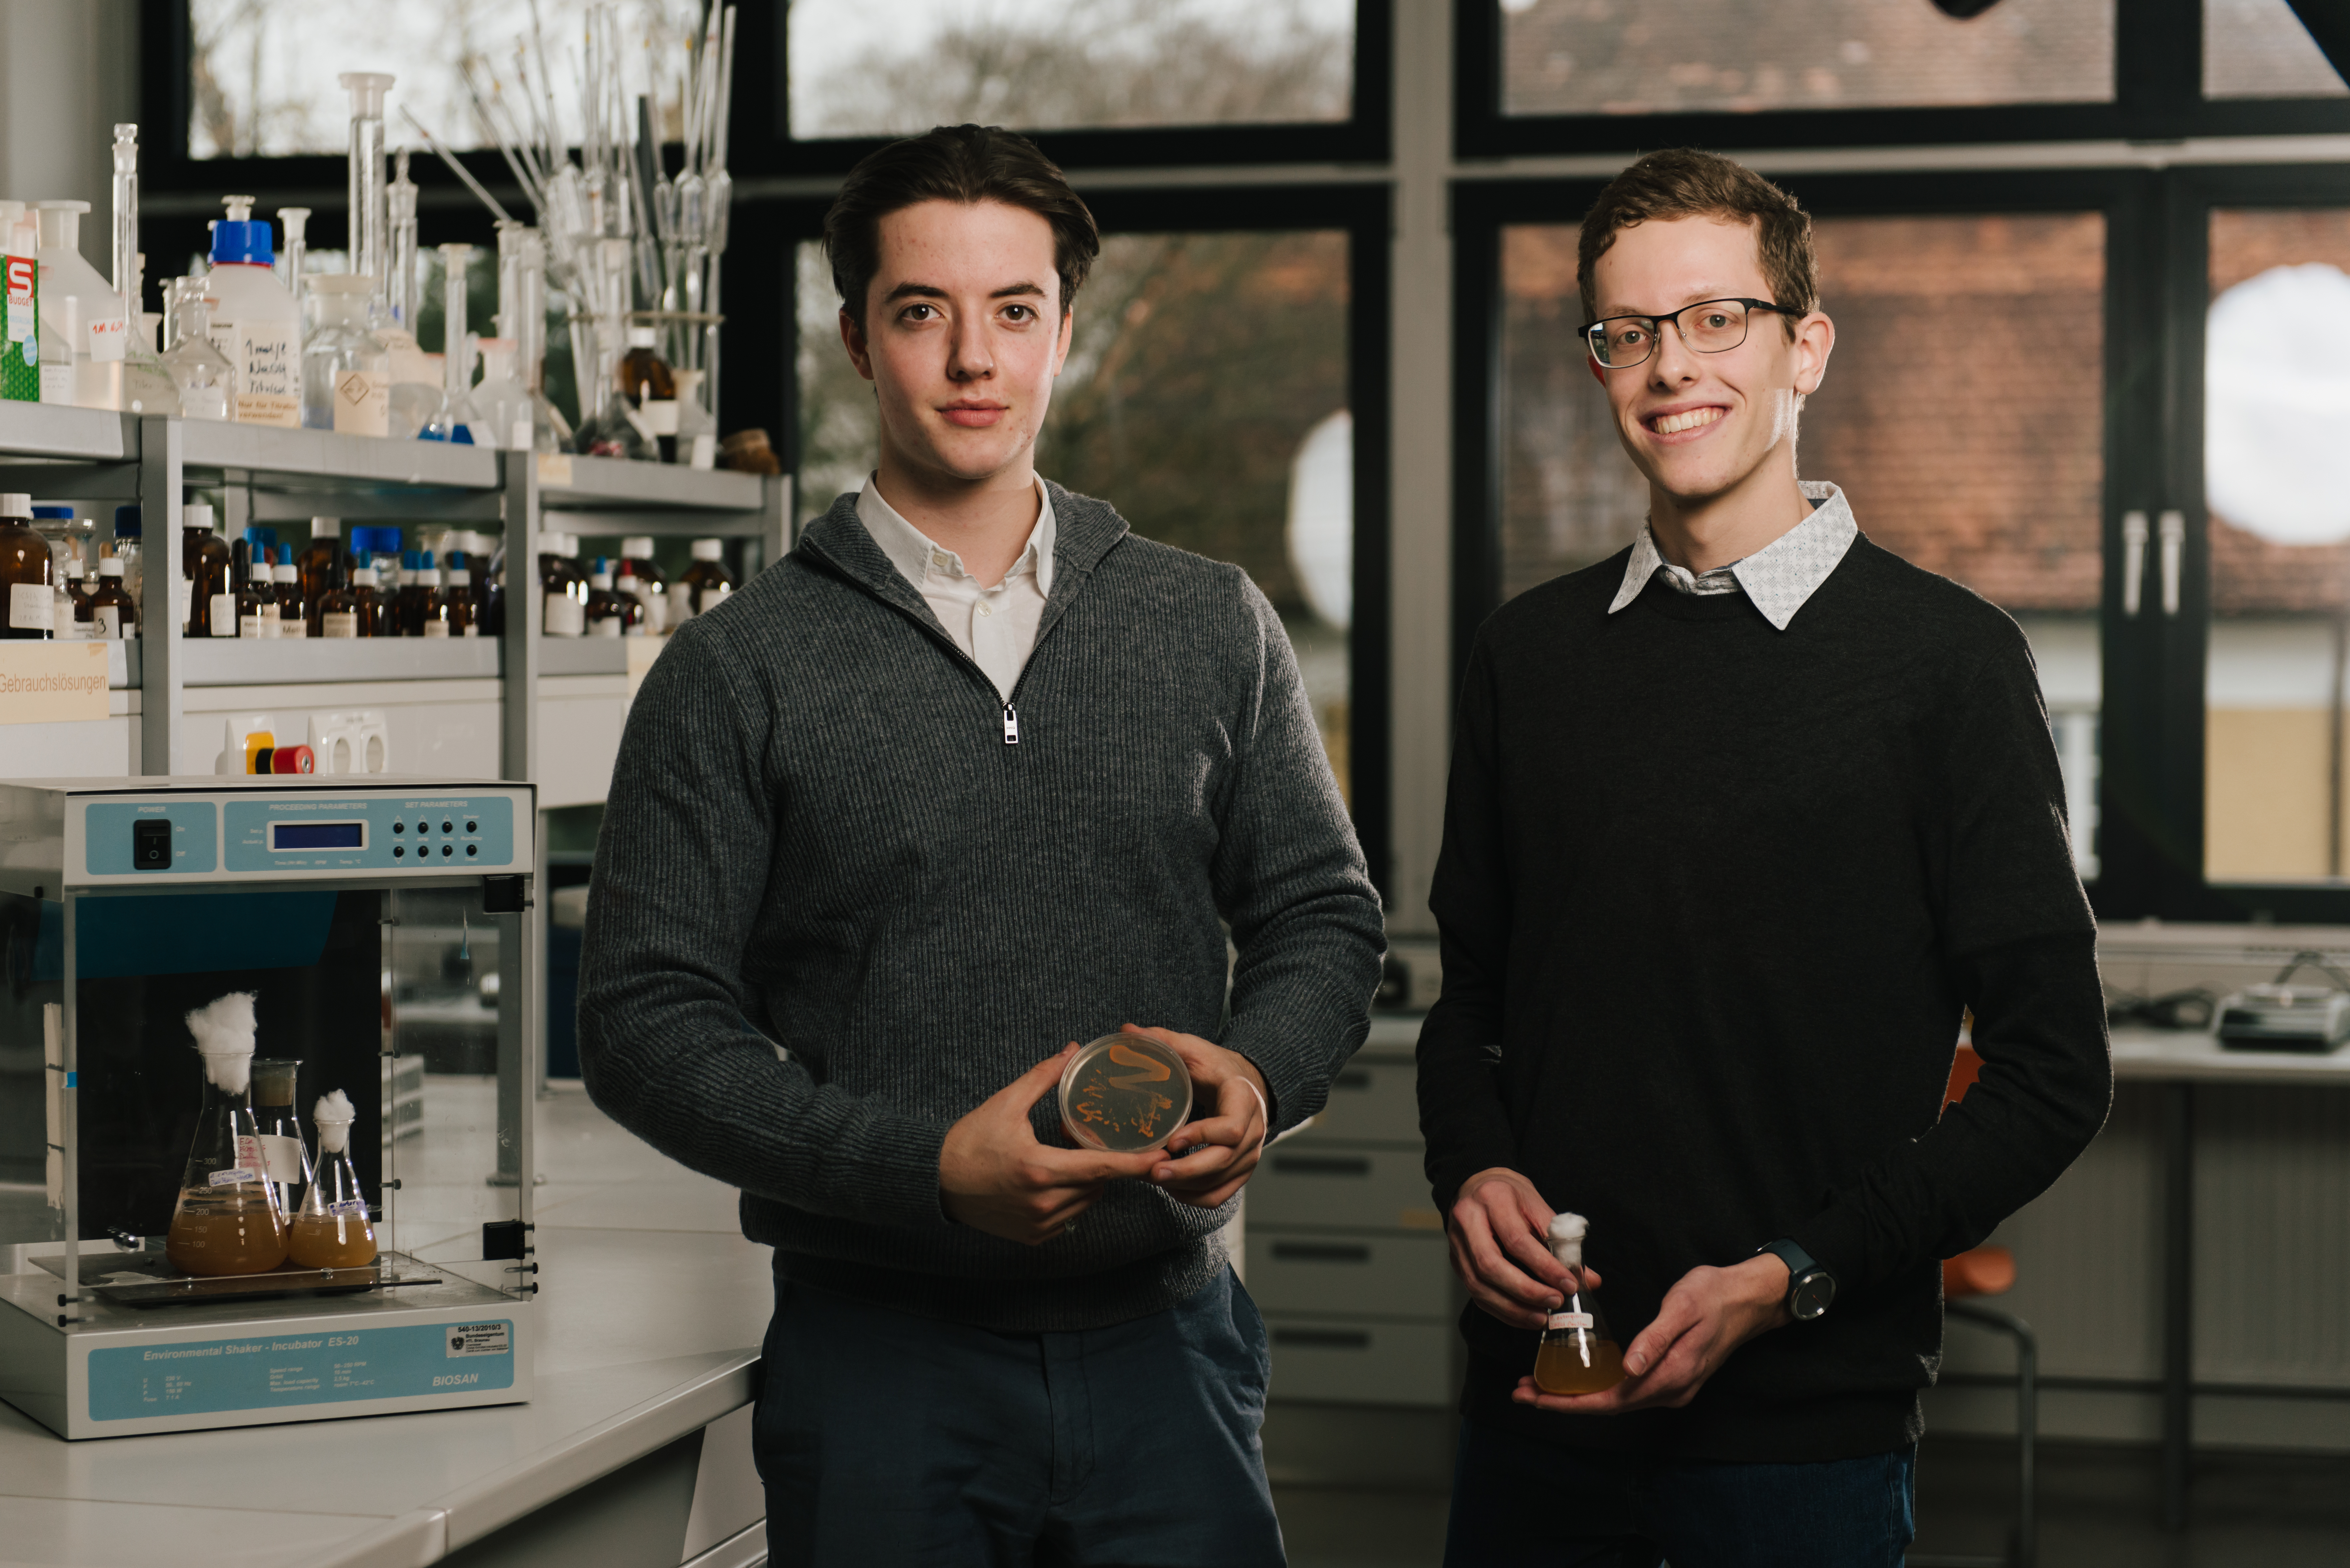
\includegraphics[width=0.75\textwidth]{./media/images/teamfoto}
    \caption{The project team}
    \label{fig:teamphoto}
\end{figure}

\newpage


\section{Timesheet}

\subsection{Tobias Daxecker}


\begin{tabularx}{\textwidth}{l p{1cm} l p{1cm} X}

    Braunau/Inn, \todayshort & & Tobias Daxecker & & \hrulefill                       \\
    \emph{Ort, Datum}        & &                 & & \emph{Unterschrift} \vspace{2cm} \\

\end{tabularx}

\subsection{Mathias Standhartinger}

\begin{tabularx}{\textwidth}{l p{1cm} l p{1cm} X}

    Braunau/Inn, \todayshort & & Mathias Standhartinger & & \hrulefill                       \\
    \emph{Ort, Datum}        & &                        & & \emph{Unterschrift} \vspace{2cm} \\

\end{tabularx}


    \chapter{Future Work\authorB{}}

To further optimize this endeavor for industrial applicability, several imperative steps must be
undertaken. Primarily, there is a critical need to augment the efficiency of bacterial proliferation and
the resultant yield of Rare Earth Elements (REEs). Achieving this entails the development of
innovative methodologies aimed at curtailing the growth duration and nutrient utilization by
Methylorubrum Extorquens. Moreover, the primary substrate for bacterial metabolism, methanol,
could be replaced with its more rudimentary and economically advantageous precursor, methane,
which is also amenable to metabolization by M. Extorquens. To realize the full-scale industrialization
of this project, rigorous testing in expansive bioreactor systems is indispensable, alongside the
incorporation of diverse forms of Electronic Waste.
Determining the most economically viable category of E-Waste necessitates extensive experimental
evaluation. Concurrently, alongside the E-Waste assessments, there arises a pressing need for the
development of a high-capacity, efficient, and durable shredding apparatus tailored to handle various
types of E-Waste. This undertaking poses multifaceted challenges, particularly in terms of safety and
cost considerations. An industrial-grade E-Waste shredder must be inherently non-combustible and
proficient in processing metal, plastic, fiberglass, and adhesive materials, all while maintaining
optimal power consumption levels and facilitating facile maintenance protocols.
    \chapter{Related Work\authorA{}}

There are some other studies that are somewhat close to our work.
Most of them have the same basic idea at their core.
That is to use \emph{M. extorquens} or lanmodulin to recycle rare earth elements.

An example for the usage of only lanmodulin would be the work of Dong et al.~\cite{originalstudy}.
Their approach was to take lanmodulin and attach it to a microbead (a small sphere made of agarose, see bottom left of figure~\ref{fig:original_study_process}).
The product of this procedure is the immobilized lanmodulin.
They made a lot of the immobilized lanmodulin and put it into a column.
Afterwards, they let a solution which contained ash from a coal power plant, which in turn contained some REEs, flow through the column.
The REEs get caught by lanmodulin, and every other metal flows freely through the whole column.
After that, they washed their column, and then they began separating the different rare earths.
They achieved this by giving solutions with different pH values into their column.
Lanmodulin releases only some certain rare earths at a certain pH which is useful for separating them.
When every rare earth has been extracted, the column can be cleaned and even be reused for the next recycling process.

\begin{figure}[H]
    \centering
    \includegraphics[width=0.8\textwidth]{./media/images/original_study_process}
    \caption{Overview of the work which inspired this thesis.
    Picture from "Bridging Hydrometallurgy and Biochemistry:
    A Protein-Based Process for Recovery and Separation of Rare Earth Elements", Dong et al.~\cite{originalstudy}.}
    \label{fig:original_study_process}
\end{figure}


This is a very clever process that even inspired this thesis.
However, this work is not easy to reproduce.
It requires costly chemicals and machinery, which only a company or a university can afford.
Therefore, it was not feasible at our school.
What must also be taken into consideration is that they used a genetically modified bacteria which produced the lanmodulin.
This step alone would take too long to achieve for a diploma thesis.

\vspace{2em}

Good et al. took another approach, which is surprisingly similar to our work.
Their basic idea was to let \emph{M. extorquens} grow in a solution which contains electronic waste (figure~\ref{fig:similar_work}) and find methods to increase the yield of this recycling method~\cite{similarwork}.
This approach is fairly similar to our own work.
However, this work did not inspire us because the paper was first published on December 27th 2023, when we already had worked three months on our project.

\begin{figure}[H]
    \centering
    \includegraphics[width=0.8\textwidth]{./media/images/similar_work}
    \caption{Very simplified abstract of the work from Good et al.
    Picture from "Scalable and Consolidated Microbial Platform for Rare Earth Element Leaching and Recovery from Waste Sources", Good et al.~\cite{similarwork}.}
    \label{fig:similar_work}
\end{figure}

The main difference to our work is their technological advantage.
They used a genetically modified strain of \emph{M. extorquens} AM1, which is called \(\Delta\)\emph{mxaF}.
They deleted the gene \emph{mxaF} to ensure that the growth of the bacteria is dependent on the uptake of rare earths.
This led to a higher rare earth uptake capacity per bacteria.

Another remarkable difference is that they did not only let the bacteria grow with crushed magnets, but also with a crushed smartphone.
This did have, interestingly, no significant impact on the growth of \emph{M. extorquens} AM1 \(\Delta\)\emph{mxaF}, according to their study.

After that, they improved the yield by adding an organic acid to the bacteria's growth medium.
This helped to extract the rare earths from the crushed magnet (and smartphone).
What also boosted their yield was that they genetically engineered \emph{M. extorquens} AM1 \(\Delta\)\emph{mxaF} even further.

We can conclude that our project was done with the minimum of resources you can use to achieve some good results.
Compared to the above-mentioned studies, we had very limited resources and only basic laboratory equipment, so we could do only basic work.
What the other studies achieved is really great, but we showed that it is possible to be part of the newest developments of science without expensive materials and equipment.
    \chapter{Conclusion\authorA{}}
The process of recycling of rare earths from e-waste using bacteria is a more eco-friendly and energy efficient way than currently established recycling methods.
In our project, we achieved to carry out this process and to determine its efficiency.
Hereby, it is important to know that we only measured the natural capacity of \emph{M. extorquens} without any additional changes.

In brief, our project can be summarized as follows:
We found a way to efficiently recycle rare earth elements from e-waste.
This works with the bacteria \emph{Methylorubrum extorquens}, which has the ability to use rare earth elements in its metabolism.
This property of the bacteria is essential because the e-waste is simply given in a crushed form to the culture medium.
The rare earths accumulate naturally in the bacteria.
The bacteria can then be opened to recover the rare earths.

\textbf{<Beschreibung von Ergebnisse / Effizienz>}

We learned a lot during the time of this project, because neither of us had previous knowledge in the field of microbiology.
This meant that we had to research everything from the ground up.
In the beginning, we thought we would do a lot of things differently than we do now.
But after three months of work, we came to a dead end because our school lacked the required equipment.
This had the consequence that we had to pivot our work in a new direction.
Afterward, we finally managed to achieve results.

The key method, which we discovered late in the project was the arsenazo-III assay.
This assay is a method to determine the concentration of rare earth elements in a sample.
Without this method, we would not have achieved any results at all, because all the other methods we tried did not work well enough.

What is also noteworthy is that we learned that at any given time something unexpected can happen, which ruins the work of a whole day.



    \appendix

    \chapter*{Acknowledgements}
\addcontentsline{toc}{chapter}{Acknowledgements}

We would like to express our gratitude for the smooth and conflict-free cooperation within our
project team.
Without it, our endeavor wouldn't have been possible.

Our supervisor, Benjamin
Seeburger M.Sc., deserves a special mention for helping us acquire all the necessary materials and
assisting us with research.

We are also thankful to Herbert Ofenmacher and Richard Sommerauer for
providing us with e-waste samples and neodymium magnets for our research.

Additionally, we would
like to thank Dipl. Ing. Andreas Scherfler and Dipl. Ing. Bernhard Schmeitzl who, despite being
supervisors of other teams, were eager to assist us with some of the problems that arose during our
project.

We would also like to extend our sincere thanks to the members of other project teams, who
were fun and engaging to be around. We would like to give a special shout-out to Robert, Jan, Emily,
Lilli, Magda, Samantha, Anna, and Mara.

We would be remiss in not mentioning the `L' key on Tobias'
keyboard, which fell victim to hours of vigorous typing for this thesis and got destroyed.

    \addcontentsline{toc}{chapter}{Listings}
    \lstlistoflistings

    \addcontentsline{toc}{chapter}{List of Figures}
    \listoffigures


    \addcontentsline{toc}{chapter}{Bibliography}
    \bibliographystyle{plain}
    \bibliography{literature}

    \chapter*{CV} \markboth{CV}{CV}
\addcontentsline{toc}{chapter}{CV}


\htlParagraph{Tobias Daxecker}

\renewcommand{\arraystretch}{1.2}
\begin{tabularx}{1\textwidth}{@{} l X l @{}}

    \emph{Geburtstag, Geburtsort:} & 25.11.2004, Braunau am Inn &
    \multirow{5}{2.5cm}{
\includegraphics[width=2.5cm]{./media/images/Daxecker}
    }
    \\
    \emph{Schulbildung:} & Volksschule Handenberg \newline Neue Mittelschule Neukirchen an der Enknach \newline HTL Braunau     & \\
    \emph{Praktika:}     & MKW Oberflächen+Draht, 4 Wochen, Produktion                                                      & \\
    & B\&R Industrial Automation, 4 Wochen, Versand                                                    & \\
    & Cloudflight, 4 Wochen, Softwareentwicklung                                                       & \\
    \emph{Anschrift:}    & Adenberg 19\newline 5144, Handenberg\newline Österreich                                          & \\
    \emph{E-Mail:}       & tobias.daxecker@htl-braunau.at                                                                   & \\

\end{tabularx}
\\\\


\htlParagraph{Mathias Standhartinger}

\begin{tabularx}{1\textwidth}{@{} l X l @{}}
    \emph{Geburtstag, Geburtsort:} & 28.12.2004, Braunau am Inn &
    \multirow{5}{2.5cm}{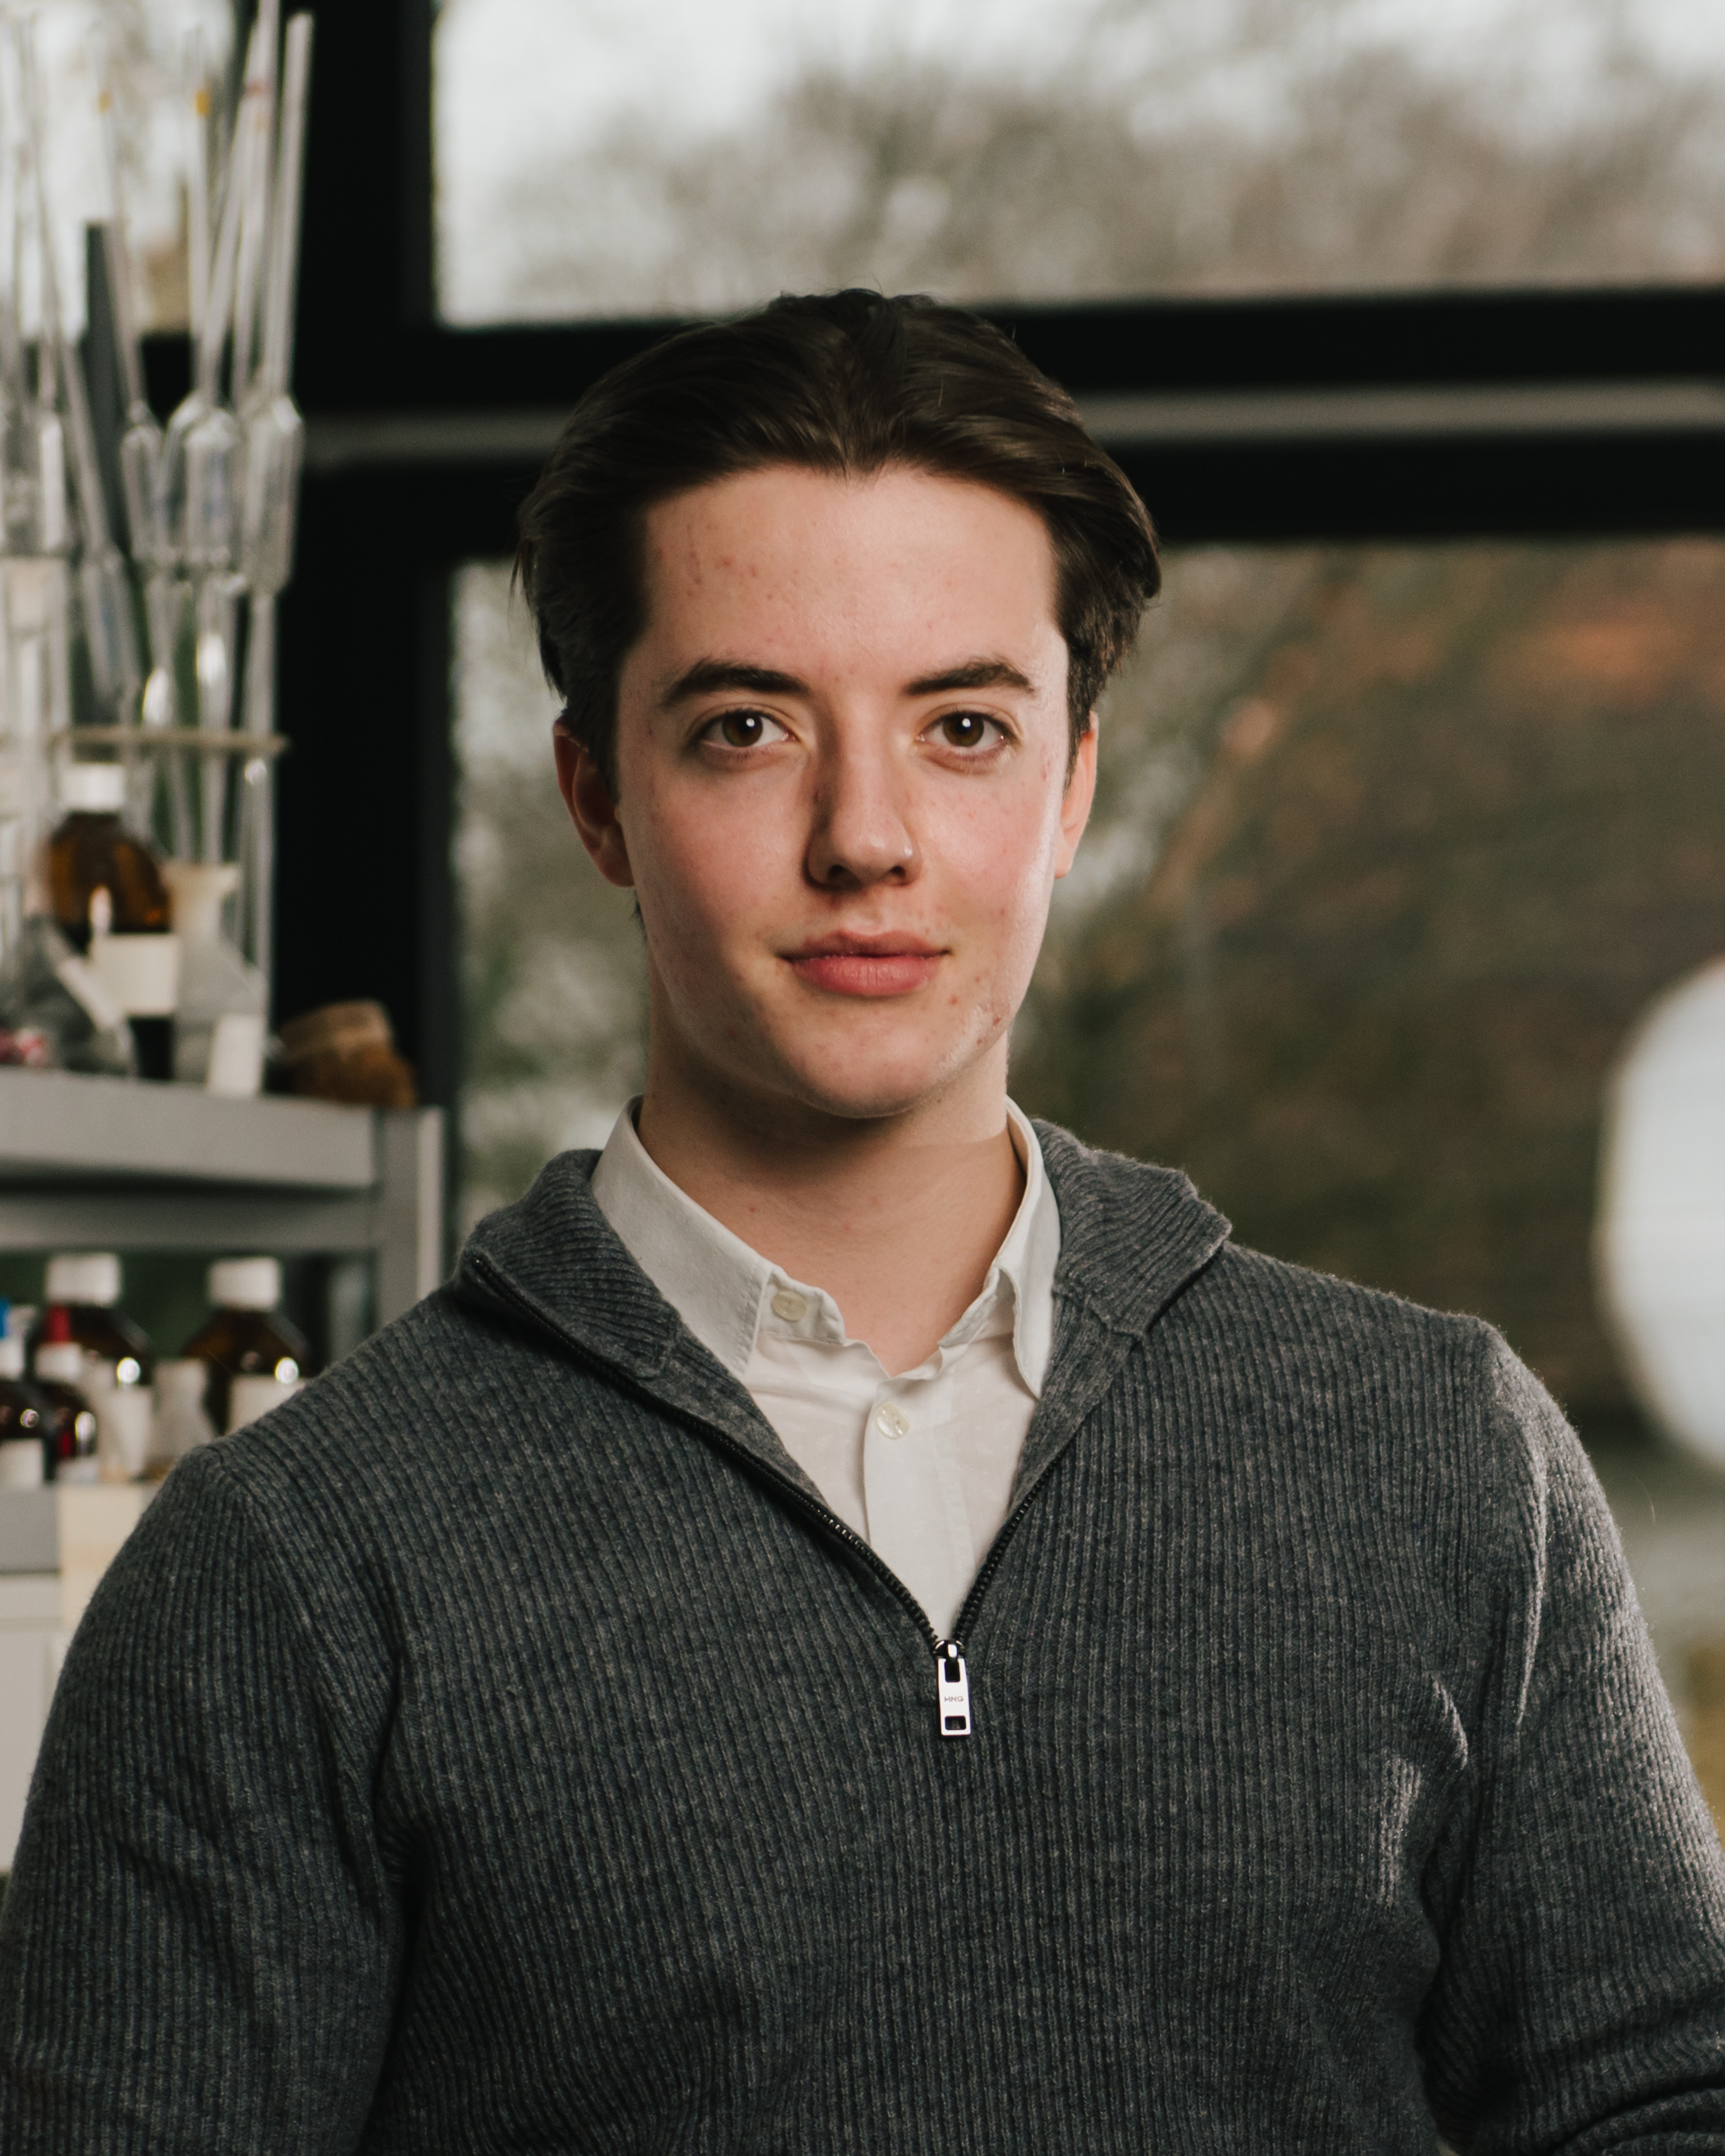
\includegraphics[width=2.5cm]{./media/images/Standhartinger}
    }
    \\
    \emph{Schulbildung:} & Volksschule Handenberg \newline Neue Mittelschule Neukirchen an der Enknach\newline HTL Braunau & \\
    \emph{Praktika:}     & brothers Klika OG, 8 Monate, Videograph, Videostratege                                          & \\
    \emph{Anschrift:}    & Polzwies 9 \newline 5143, Schwand im Innkreis\newline Österreich                                              & \\
    \emph{E-Mail:}       & m.standhartinger@htl-braunau.at                                                                 & \\

\end{tabularx}



\end{document}